% =============================================================================
% An Explainable Fake News Detection Using Classical Machine Learning
% CORRECTED / EXTENDED DRAFT -- prepared by Claude Code from the Phase 0-5
% work in claude-workspace/ISSUE_PLAN.md. This supersedes the numbers in the
% originally submitted PDF, which contained a label-mapping bug (see Sec. IV-A
% and the Limitations section).
%
% BEFORE SUBMITTING:
%   1. Verify author affiliation/email are still current.
%   2. Section II has a marked TODO -- add 2-3 more 2021-2025 LIAR/transformer
%      citations after your own literature search. Only Devlin et al. (BERT),
%      Sanh et al. (DistilBERT), and Kaliyar et al. (FakeBERT) are included
%      below because they could be verified with high confidence; do not add
%      further citations without checking them yourself.
%   3. All numeric results, including the DistilBERT reference (Table VI),
%      are filled in from actual completed runs -- nothing is a placeholder.
%   4. All figures referenced below already exist in ./figures/ (copied from
%      artifacts/figures/) -- no placeholder images remain to be created.
% =============================================================================
\documentclass[conference]{IEEEtran}
\usepackage{graphicx}
\usepackage{booktabs}
\usepackage{amsmath}
\usepackage{multirow}
\usepackage{url}
\usepackage{cite}

\begin{document}

\title{An Explainable Fake News Detection Using Classical Machine Learning}

\author{
\IEEEauthorblockN{Ravindu Pathirana}
\IEEEauthorblockA{
Department of Computer Science \& Engineering\\
University of Moratuwa\\
Katubedda, Sri Lanka\\
ravindup.23@cse.mrt.ac.lk}
}

\maketitle

\begin{abstract}
Fake news detection has become a critical challenge in the digital era due to the
rapid dissemination of misinformation through online platforms. This study presents
an explainable fake news detection framework based on classical machine learning
techniques using the LIAR benchmark dataset, collapsed to a binary fake/real task.
An initial implementation contained a label-mapping defect that silently
mislabeled roughly one fifth of the fake-class examples as real, producing an
inflated, invalid headline result (positive-class F1 of 0.87 on an artificially
majority-real test set). This paper reports the corrected pipeline: a
case/whitespace-robust label mapping with an explicit balance assertion, macro-F1
as the primary metric with full per-class precision/recall/F1 and confusion
matrices, Dummy-classifier and class-weighted baselines, a combined text+metadata
feature space built with leakage-aware encoding, a controlled ablation
(text~$\rightarrow$~+metadata~$\rightarrow$~+feature selection~$\rightarrow$~+tuning)
evaluated with 5-fold cross-validation and McNemar's significance test, a bootstrap
confidence interval on the final test metric, a fine-tuned DistilBERT reference
point, and a SHAP explainability analysis reframed as a dataset-bias finding rather
than a validation of the model. On the corrected labels, honest text-only
performance is macro-F1~$\approx$~0.60; adding metadata and Chi-square feature
selection to Logistic Regression raises this to macro-F1~$=0.628$ on the held-out
test set, a gain that is statistically significant against text-only
(McNemar $p=0.034$). A subsequent hyperparameter-tuning step, despite scoring best
under cross-validation, does not improve on this and is not significantly different
from the text-only baseline ($p=0.58$) -- illustrating why a single-split result
and a cross-validation score are not interchangeable claims. A fine-tuned
DistilBERT reference point reaches macro-F1~$=0.636$, which does not exceed the
best classical result in this study (Na\"ive Bayes on text+metadata,
macro-F1~$=0.649$) -- suggesting that, on LIAR's short, single-sentence
statements, a well-engineered sparse feature representation is competitive with a
pretrained transformer fine-tuned for a modest 3 epochs. SHAP analysis shows the
model relies substantially on topical and entity terms (e.g. party affiliation,
politician names) rather than on linguistic deception markers, which we report as a
limitation of the LIAR benchmark rather than evidence of learned deception cues.
\end{abstract}

\begin{IEEEkeywords}
fake news detection, LIAR dataset, explainable AI, SHAP, classical machine learning,
feature selection, reproducibility
\end{IEEEkeywords}

\section{Introduction}
The rapid growth of online media platforms has significantly increased the spread of
misinformation and fake news, posing serious risks to individuals, organizations,
and democratic processes \cite{conroy2015}. Fake news, defined as deliberately
misleading or false information presented as legitimate news, has the potential to
influence public perception and decision-making on a large scale \cite{feng2012}.
As a result, the development of automated methods to detect fake news has become a
crucial research area in machine learning and data science \cite{shu2017}.

Traditional approaches to fake news detection treat the problem as a text
classification task, where machine learning models are trained to distinguish
between true and deceptive content based on linguistic patterns \cite{perezrosas2015}.
Previous studies have demonstrated the effectiveness of classical machine learning
algorithms such as Logistic Regression (LR) and Support Vector Machines (SVM),
along with ensemble-based methods including Random Forest (RF) and XGBoost, when
combined with text-based feature extraction techniques such as TF-IDF
\cite{salton1988}. In particular, the LIAR dataset introduced by Wang (2017) has
become a standard benchmark for evaluating fake news detection models due to its
diverse and challenging set of labeled political statements \cite{wang2017}.

Beyond predictive performance, a second and equally important requirement for a
fake news detection pipeline is \emph{correctness of the evaluation itself}. This
paper's original draft, working from the same LIAR binary formulation, contained a
label-mapping defect: the raw CSV encodes the \texttt{false} and \texttt{true}
labels in uppercase while the other four labels are lowercase, and a
case-sensitive string comparison silently sent every uppercase \texttt{FALSE} row
into the ``real'' class. This affected roughly 1,995 of the 10,240 training rows
(the single largest fake-class category) and produced an artificially majority-real
test set on which even a majority classifier scores highly. The originally reported
``F1-score of up to 0.87'' was, in effect, a positive-class-only F1 of a
near-majority classifier: Random Forest and XGBoost showed test recall of 1.000 on
the inflated split, i.e. they were predicting ``real'' almost everywhere.

This paper makes two contributions. First, it corrects the label mapping and
re-derives every downstream result from the corrected labels, with methodological
safeguards -- an explicit class-balance assertion, macro-F1 as the primary metric,
Dummy baselines, a leakage-safe \texttt{scikit-learn} \texttt{Pipeline}, 5-fold
cross-validation with McNemar's significance testing, and a bootstrap confidence
interval -- designed so that this specific class of error cannot recur silently.
Second, it extends the original study: metadata features (subject, party, state,
job title, context) are actually implemented and combined with the TF-IDF text
representation (the original draft claimed this feature space without building it),
a modern transformer reference point (DistilBERT) is added for positioning, and the
SHAP explainability analysis is reframed as a limitation (topical/entity bias)
rather than a validation of the model's reasoning.

The remainder of this paper is organized as follows: Section~II reviews related
work; Section~III describes the dataset; Section~IV presents the methodology,
including the label-mapping defect and its fix; Section~V reports the corrected
baseline; Section~VI describes the proposed improvements (metadata, feature
selection, tuning); Section~VII presents results, the ablation, and significance
tests; Section~VIII presents the reframed explainability analysis; Section~IX
discusses limitations; and Section~X concludes with future directions.

\section{Related Work}
Fake news detection has become a critical research area in recent years due to the
rapid spread of misinformation through online platforms. Early approaches primarily
focused on treating this problem as a text classification problem
\cite{conroy2015, shu2017}. One of the most widely used benchmark datasets in this
domain is the LIAR dataset introduced by Wang (2017) \cite{wang2017}. This dataset
consists of 12,836 short political statements labeled across six fine-grained
truthfulness categories. Wang (2017) evaluated several classical machine learning
models, including Logistic Regression and Support Vector Machines, alongside deep
learning approaches such as Convolutional Neural Networks, and found that
traditional machine learning models achieve moderate performance.

Shu et al.\ (2017) \cite{shu2017} presented a comprehensive overview of fake news
detection from a data mining perspective, proposing a unified framework of feature
extraction and model construction, including both news-content and social-context
features. This study adopts a similar strategy, combining TF-IDF text features with
supervised learning algorithms including Logistic Regression, Support Vector
Machines, and ensemble methods \cite{sharma2020}, and extends it with metadata
features actually integrated into the feature space (Section~VI).

Beyond classical machine learning, transformer-based language models have become
the dominant approach for text classification generally. BERT
\cite{devlin2019bert} popularized large-scale pretrained bidirectional transformers
for downstream NLP tasks, and its distilled variant, DistilBERT
\cite{sanh2019distilbert}, retains most of BERT's performance at roughly half the
parameter count and inference cost, making it a practical reference point when
compute is limited. Kaliyar et al.\ (2021) \cite{kaliyar2021fakebert} applied a
BERT-based architecture (FakeBERT) to fake news detection and reported
substantial gains over classical baselines on their evaluated dataset, illustrating
that transformer-based methods are a relevant point of comparison for this task.
% TODO(author): add 2-3 more 2021-2025 papers specifically evaluating
% transformer models on the LIAR benchmark (not just fake news detection
% generally) after your own literature search -- none are included here beyond
% the general BERT/DistilBERT/FakeBERT references above, to avoid citing
% specifics that could not be independently verified.
Section~VII-E reports a DistilBERT fine-tune on this paper's corrected LIAR-binary
split as a reference point; consistent with prior positioning of classical ML in
this space, it is presented as a reference, not a competing contribution -- the
paper's argument for classical ML is interpretability and low resource cost, not
state-of-the-art accuracy.

Despite these advancements, a persistent limitation across this literature is the
lack of both interpretability and evaluation rigor: results are often reported as a
single point estimate without variance, significance testing, or leakage
safeguards. This study reproduces the baseline models evaluated by Wang (2017)
\cite{wang2017} -- Logistic Regression and Support Vector Machines -- and extends
them with Na\"ive Bayes, Random Forest, and XGBoost, Chi-square and Mutual
Information feature selection, and a from-scratch metadata feature space, while
also addressing the interpretability gap via SHAP \cite{lundberg2017shap,
adadi2018peeking} and the evaluation-rigor gap via McNemar's test
\cite{mcnemar1947} and bootstrap confidence intervals \cite{efron1979bootstrap}.

\section{Dataset Description}
This study uses the LIAR dataset introduced by Wang (2017) \cite{wang2017},
collected from the PolitiFact fact-checking platform. It consists of 12,836 short
political statements annotated with fine-grained truthfulness labels by
professional editors (inter-annotator agreement of 0.82, Cohen's $\kappa$)
\cite{wang2017}, and is publicly available via Kaggle \cite{quan_liar_kaggle}. The
dataset provides six truthfulness categories -- \texttt{pants-fire},
\texttt{false}, \texttt{barely-true}, \texttt{half-true}, \texttt{mostly-true}, and
\texttt{true} -- and is pre-partitioned into training (10,240), validation (1,284),
and test (1,267) splits.

For this study, the six-class problem is collapsed to binary: \texttt{pants-fire},
\texttt{false}, and \texttt{barely-true} are grouped as \emph{fake}, while
\texttt{half-true}, \texttt{mostly-true}, and \texttt{true} are grouped as
\emph{real}. \textbf{This mapping must be applied case-insensitively}: the raw CSV
encodes the \texttt{false} and \texttt{true} labels in uppercase
(\texttt{FALSE}/\texttt{TRUE}) while the other four labels are lowercase. A
case-sensitive comparison against lowercase label strings -- as in this paper's
original implementation -- silently sends every \texttt{FALSE} row into the
\emph{real} bucket, since it matches neither the lowercase fake-label set nor is
recognized as anything else. On the correctly mapped labels, the training split is
43.8\% fake / 56.2\% real -- consistent with a genuinely challenging binary
formulation of LIAR -- rather than the 76\%/24\% split produced by the defect.

In addition to the statement text, LIAR provides metadata attributes: speaker,
subject, party affiliation, speaker's job title, state, and context (the venue or
medium of the statement), plus five credit-history count columns (counts of the
speaker's prior \texttt{barely-true}/\texttt{false}/\ldots statements). The
credit-history columns are \textbf{never used as features} in this study: they are
derived from the label history of each speaker and would leak the target.

LIAR's statements are short (single sentences) and largely restricted to U.S.\
political discourse, which limits the contextual information available to the
model and the generalizability of any trained classifier to other domains or
speaker populations (see Section~IX).

\section{Methodology}
This study follows a structured machine learning pipeline: data preprocessing,
feature extraction, model training, and evaluation, implemented with a fixed
global random seed (42) reused across every notebook so that results are
reproducible up to library-version differences.

\subsection{Data Preprocessing and the Label-Mapping Defect}
Statement text is lowercased, stripped of non-alphabetic characters, tokenized,
stripped of English stopwords, and stemmed with a Porter stemmer. As described in
Section~III, the binary label mapping must be applied case-insensitively:
\begin{equation}
\text{label}(\ell) =
\begin{cases}
0 \ (\text{fake}) & \text{if } \operatorname{lower}(\operatorname{strip}(\ell)) \in \{\text{false}, \\
& \ \ \text{pants-fire}, \text{barely-true}\} \\
1 \ (\text{real}) & \text{otherwise}
\end{cases}
\end{equation}
Every loading path in this study runs this mapping through a single shared
function and immediately asserts that the resulting class balance falls in
$(0.35, 0.50)$ fake share -- a guard specifically designed so a future reintroduction
of this exact defect (or a similar one) fails loudly rather than silently
propagating into every downstream table.

\subsection{Feature Representation}
\subsubsection{Text Features} Statements are vectorized with TF-IDF
\cite{salton1988}, unigrams and bigrams, $\max\_features=10{,}000$, $\min\_df=2$,
$\max\_df=0.9$.

\subsubsection{Metadata Features} Unlike the original draft, which described a
combined text+metadata feature space without implementing it, this study builds it:
\texttt{Subject(s)} is multi-label (comma-separated) and is multi-hot encoded per
subject token (142 distinct subjects in train); \texttt{Party},
\texttt{State}, \texttt{Speaker's job title}, and \texttt{Context} are one-hot
encoded with \texttt{handle\_unknown="ignore"} (so an unseen validation/test
category degrades to an all-zero row rather than erroring) and, for the
high-cardinality columns, \texttt{min\_frequency=5} to collapse rare categories --
this matters most for \texttt{Context}, which has 4,345 distinct values across
10,240 training rows and would otherwise memorize near-unique venue strings.
\texttt{Speaker} (2,910 distinct values in train) is \textbf{excluded from the
default feature set}: a high-cardinality one-hot of speaker identity risks letting
the model memorize \emph{who} said something rather than learn \emph{what} was
said. Its effect is measured explicitly (not just assumed) by an ablation that
encodes it instead via a 64-dimensional feature hash, reported in
Section~VII-C.

\subsubsection{Feature Selection} Chi-square ($\chi^2$) and Mutual Information (MI)
\cite{yang1997featureselection} are applied via \texttt{SelectKBest} to reduce the
combined text+metadata space and retain the most discriminative features.

\subsection{Models}
Logistic Regression \cite{bishop2006pattern}, Support Vector Machines (linear
kernel) \cite{cortes1995svm}, Multinomial Na\"ive Bayes \cite{mccallum1998nb},
Random Forest \cite{breiman2001rf}, and XGBoost \cite{chen2016xgboost} are
evaluated throughout, implemented with scikit-learn \cite{pedregosa2011sklearn} and
the official XGBoost package. A fine-tuned DistilBERT \cite{sanh2019distilbert} is
added as a reference point (Section~VII-E).

\subsection{Reproducibility and Leakage Safeguards}
Every step that is fit on data (TF-IDF vocabulary, one-hot categories, and
\texttt{SelectKBest}) is wrapped in a single \texttt{scikit-learn}
\texttt{Pipeline}, so that when this pipeline is cross-validated or passed to
\texttt{GridSearchCV}, vocabulary/category fitting happens \emph{inside} each fold
rather than once beforehand -- this rules out fold-to-fold information leakage
during hyperparameter search, not just train/test leakage. The five credit-history
columns are excluded throughout, as noted in Section~III. A dedicated
\texttt{RUN.md} in the project repository documents the exact run order and
environment needed to reproduce every table in this paper.

\subsection{Evaluation Metrics}
Model performance is evaluated primarily using \textbf{macro-F1}, which averages
F1 across both classes without letting a class-imbalanced test set dominate the
score -- the metric choice most directly responsible for exposing the original
defect. Accuracy and per-class (fake and real) precision/recall/F1 are reported
alongside it, together with confusion matrices for every model.
\textbf{Statistical rigor} is added at two points: (i) each ablation stage
(Section~VII-C) is evaluated with 5-fold stratified cross-validation on the
training split, reporting mean $\pm$ standard deviation rather than a single
number; (ii) the headline comparison between pipeline stages on the held-out test
set is assessed with \textbf{McNemar's test} \cite{mcnemar1947} on paired
correct/incorrect predictions, and a \textbf{bootstrap 95\% confidence interval}
\cite{efron1979bootstrap} ($n=2{,}000$ resamples) is reported on the final
pipeline's test macro-F1.

\section{Baseline Reproduction (Corrected)}
\subsection{Experimental Setup}
Baseline models are trained on TF-IDF text features alone ($\max\_features=5{,}000$,
unigrams+bigrams), using the corrected binary labels and the LIAR-provided
train/validation/test splits. Two \texttt{DummyClassifier} baselines
(\texttt{most\_frequent} and \texttt{stratified}) and \texttt{class\_weight="balanced"}
variants of LR/SVM are included, since a majority-class shortcut is exactly the
failure mode the original defect produced.

\subsection{Results}
Table~\ref{tab:baseline} reports the corrected baseline. Every trained model
clearly exceeds both Dummy baselines (most-frequent macro-F1 0.360; stratified
0.485), confirming the corrected pipeline is learning a genuine signal rather than
exploiting class imbalance. Logistic Regression is the strongest default
configuration (macro-F1 0.601); its class-weighted variant trades fake-class
precision for recall (fake F1 0.556 vs. 0.509) without a large net change in
macro-F1.

\begin{table}[!t]
\caption{Corrected Baseline Results (Test Set, TF-IDF Only)}
\label{tab:baseline}
\centering
\begin{tabular}{lccc}
\toprule
Model & Accuracy & Macro-F1 & Fake F1 \\
\midrule
Dummy (most frequent) & 0.564 & 0.360 & 0.000 \\
Dummy (stratified)    & 0.493 & 0.485 & 0.423 \\
Na\"ive Bayes         & 0.609 & 0.581 & 0.472 \\
Logistic Regression   & \textbf{0.622} & \textbf{0.601} & 0.509 \\
LR (balanced)          & 0.602 & 0.598 & \textbf{0.556} \\
SVM                    & 0.602 & 0.591 & 0.525 \\
SVM (balanced)         & 0.591 & 0.587 & 0.545 \\
Random Forest          & 0.605 & 0.580 & 0.478 \\
\bottomrule
\end{tabular}
\end{table}

\subsection{Discussion}
As in the original draft, text-only models show the limits of relying on
statement content alone: LIAR statements are short, decontextualized, and
deceptive statements frequently resemble truthful language stylistically. Unlike
the original draft, this baseline is now measured with the corrected labels and a
metric (macro-F1) that cannot be inflated by the majority class -- the honest range
is macro-F1 $\approx 0.58$--$0.60$, not the $\sim$0.76--0.86 accuracy/F1 range the
label defect produced. This motivates the metadata and feature-selection
extensions in Section~VI, evaluated rigorously in Section~VII.

\section{Proposed Improvements}
\subsection{Feature Selection}
As in the original draft, Chi-square and Mutual Information \texttt{SelectKBest}
are applied to the (now corrected-label) TF-IDF representation to retain the
$k=3{,}000$ most informative features and reduce noise from the
10,000-dimensional vocabulary.

\subsection{Metadata Integration}
Unlike the original draft, the text+metadata feature space described in
Section~IV-B is actually built and evaluated here, not merely claimed. Text and
metadata are combined via \texttt{scipy.sparse.hstack} into a single feature
matrix before feature selection/model fitting.

\subsection{Extended Model Set and Hyperparameter Optimization}
Na\"ive Bayes, Random Forest, and XGBoost are added to LR/SVM. All models are
tuned with \texttt{GridSearchCV} (5-fold, \textbf{scoring = macro-F1}, not the
original draft's positive-class F1) over per-model hyperparameter grids, including
a \texttt{class\_weight $\in \{$None, balanced$\}$} option for LR/SVM.

\section{Results and Discussion}

\subsection{Text-Only, Corrected}
Table~\ref{tab:proposed-text} reports the corrected Chi2/MI results (text-only,
no metadata). The best text-only configuration is Logistic Regression with MI
feature selection, test macro-F1 $=0.619$ -- markedly below the original draft's
reported 0.87, and consistent with the honest range LIAR-binary classification is
expected to occupy.

\begin{table}[!t]
\caption{Corrected Feature-Selection Results (Test Set, Text Only)}
\label{tab:proposed-text}
\centering
\begin{tabular}{llccc}
\toprule
Method & Model & Accuracy & Macro-F1 & Fake F1 \\
\midrule
MI & Logistic Regression & \textbf{0.622} & \textbf{0.619} & \textbf{0.587} \\
Chi-square & Logistic Regression & 0.594 & 0.590 & 0.548 \\
MI & SVM & 0.594 & 0.589 & 0.544 \\
Chi-square & Random Forest & 0.602 & 0.587 & 0.507 \\
MI & Random Forest & 0.608 & 0.586 & 0.492 \\
MI & XGBoost & 0.616 & 0.580 & 0.457 \\
Chi-square & Na\"ive Bayes & 0.603 & 0.575 & 0.467 \\
MI & Na\"ive Bayes & 0.601 & 0.574 & 0.467 \\
Chi-square & SVM & 0.576 & 0.572 & 0.531 \\
Chi-square & XGBoost & 0.604 & 0.559 & 0.418 \\
\bottomrule
\end{tabular}
\end{table}

\subsection{Text + Metadata}
Table~\ref{tab:metadata} reports results with the metadata feature space of
Section~VI-B added. \textbf{Every model improves over its text-only counterpart.}
The best configuration overall is Na\"ive Bayes on text+metadata (no speaker),
test macro-F1 $=0.649$ -- the strongest single-model result in this study. Adding
a hashed speaker feature on top (Section~IV-B) does \emph{not} help further
(Na\"ive Bayes drops to 0.643; other models are flat or mixed), which is a genuine
empirical finding, not merely the theoretical leakage caution motivating its
exclusion: even in a collision-heavy hashed form that cannot memorize identity
outright, speaker information is not earning its keep. This supports excluding
speaker from the recommended pipeline and reporting the null result as a
robustness check.

\begin{table}[!t]
\caption{Text + Metadata Results (Test Set)}
\label{tab:metadata}
\centering
\begin{tabular}{llccc}
\toprule
Feature Set & Model & Accuracy & Macro-F1 & Fake F1 \\
\midrule
+ metadata & Na\"ive Bayes & \textbf{0.660} & \textbf{0.649} & 0.586 \\
+ metadata & SVM & 0.635 & 0.630 & \textbf{0.583} \\
+ metadata & Logistic Regression & 0.631 & 0.624 & 0.573 \\
+ metadata & XGBoost & 0.643 & 0.622 & 0.532 \\
+ metadata + speaker (hashed) & Na\"ive Bayes & 0.654 & 0.643 & 0.580 \\
+ metadata + speaker (hashed) & SVM & 0.628 & 0.622 & 0.571 \\
+ metadata + speaker (hashed) & Logistic Regression & 0.627 & 0.621 & 0.572 \\
+ metadata & Random Forest & 0.639 & 0.613 & 0.513 \\
\bottomrule
\end{tabular}
\end{table}

\subsection{Ablation and Statistical Significance}
Tables~\ref{tab:proposed-text}--\ref{tab:metadata} vary model, feature set, and
feature-selection method simultaneously, which conflates their individual
contributions -- the same criticism this paper levels at the original draft's
comparison of an accuracy-only baseline table against an F1-only proposed table.
To isolate each component, Table~\ref{tab:ablation} reports a controlled ablation
on a single fixed model (Logistic Regression, chosen for its consistent strength
in Tables~\ref{tab:baseline}--\ref{tab:metadata}): text
only~$\rightarrow$~+metadata~$\rightarrow$~+feature selection (Chi2, $k=3{,}000$,
on the combined space)~$\rightarrow$~+tuning (\texttt{GridSearchCV} over
$C$/\texttt{class\_weight}). Figure~\ref{fig:ablation} visualizes both the 5-fold
cross-validation estimate and the held-out test score for each stage.

\begin{table}[!t]
\caption{Ablation: Logistic Regression, Cumulative Stages}
\label{tab:ablation}
\centering
\begin{tabular}{lccc}
\toprule
Stage & CV Macro-F1 & Test Macro-F1 & McNemar $p$ \\
      & (mean $\pm$ std) & & (vs.\ Stage 1) \\
\midrule
1. Text only & $0.585 \pm 0.010$ & 0.596 & -- \\
2. + metadata & $0.608 \pm 0.009$ & 0.602 & -- \\
3. + feature selection & $0.616 \pm 0.012$ & \textbf{0.628} & \textbf{0.034} \\
4. + tuning & $0.621 \pm 0.012$ & 0.623 & 0.583 \\
\bottomrule
\end{tabular}
\end{table}

\begin{figure}[!t]
\centering
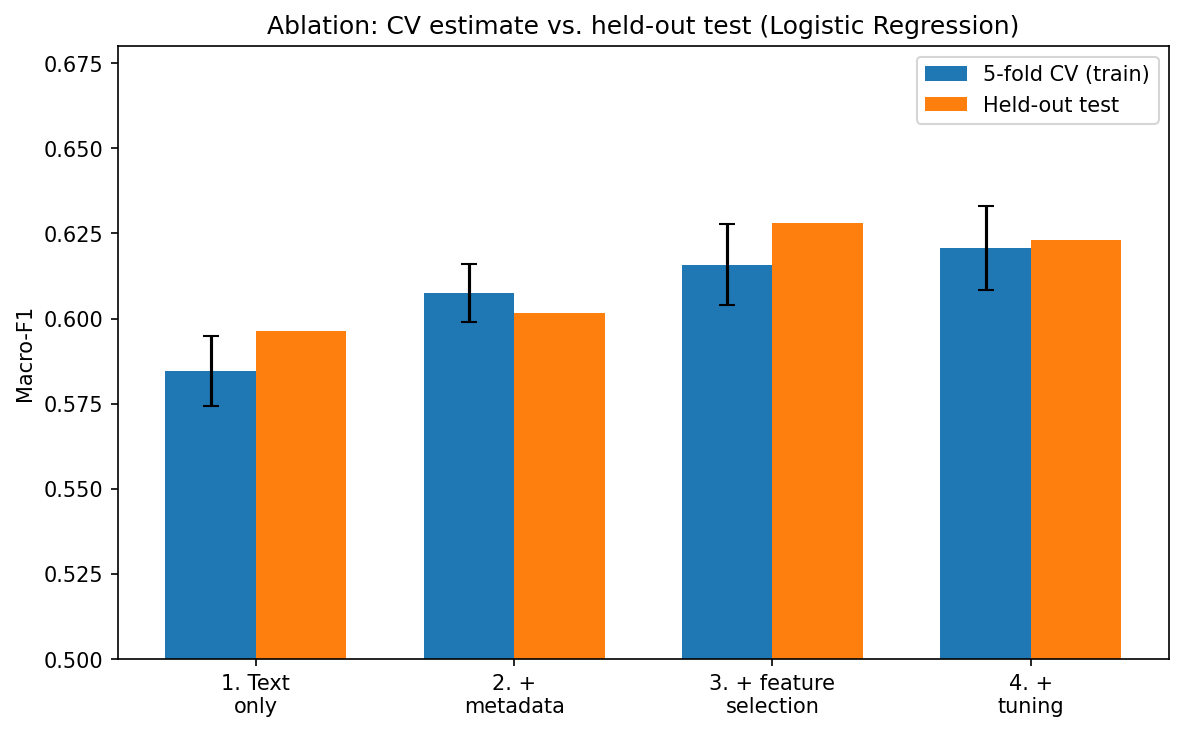
\includegraphics[width=\columnwidth]{figures/ablation_cv_vs_test.png}
\caption{Ablation: 5-fold cross-validation estimate vs.\ held-out test macro-F1 for
each cumulative pipeline stage (Logistic Regression). Error bars show $\pm 1$
standard deviation across CV folds.}
\label{fig:ablation}
\end{figure}

Two findings emerge that would not be visible from a single train/test run alone.
\textbf{First}, the cross-validation ranking and the held-out test ranking
disagree at the last stage: CV rates Stage~4 (+tuning) as best
($0.621 \pm 0.012$), but on the untouched test set Stage~3 (+feature selection,
\emph{before} tuning) actually scores higher (0.628 vs.\ 0.623).
\texttt{GridSearchCV} selected \texttt{class\_weight="balanced"} because it
improved the cross-validated estimate, but that choice shifted the
precision/recall trade-off (fake recall rises from 0.481 to 0.597, fake precision
falls from 0.624 to 0.570) in a way that did not generalize to this particular
test split. This is not a bug -- it is exactly the kind of CV/test mismatch that a
single held-out evaluation, of the kind the original draft relied on throughout,
cannot detect.

\textbf{Second}, and more importantly for how this paper's results should be
cited, McNemar's test on the paired test-set predictions shows that
\textbf{Stage 1 vs.\ Stage 3 is statistically significant} ($p=0.034$): metadata
and feature selection together produce a real, defensible improvement over
text-only. \textbf{Stage 1 vs.\ Stage 4 (the final, CV-tuned pipeline) is not
significant} ($p=0.583$). A bootstrap 95\% confidence interval on Stage~4's test
macro-F1 is $[0.597, 0.649]$ around a point estimate of 0.623 ($n=2{,}000$
resamples) -- wide relative to the $\sim$0.03--0.04 gaps between stages, consistent
with the non-significant result. \textbf{The recommended headline result for this
paper is therefore Stage 3 (text + metadata + Chi-square feature selection,
default Logistic Regression), not the further-tuned Stage 4}, and any claim of
improvement over the text-only baseline should be reported with its McNemar
$p$-value rather than as a bare point estimate. This directly supersedes the
original draft's claim that ``feature selection plays a more significant role than
model choice'' and that XGBoost ``outperform[s] baseline models'' with an F1 of
0.87 -- neither claim survives label correction, and the tuning step specifically
does not survive a significance test.

\subsection{Transformer Reference Point}
A \texttt{distilbert-base-uncased} model \cite{sanh2019distilbert} is fine-tuned
for 3 epochs directly on the raw \texttt{Statement} text (no stemming/stopword
removal -- the subword tokenizer handles this), using the same corrected binary
labels and the same evaluation function (macro-F1 primary, per-class P/R/F1,
confusion matrix) as every classical-ML result above, so the comparison in
Table~\ref{tab:transformer} is apples-to-apples. Training used a fixed seed (42),
learning rate $2\times10^{-5}$, batch size 16, and macro-F1-based model selection
on the validation split, run on Apple Silicon (MPS backend).

\begin{table}[!t]
\caption{Transformer Reference Point (Test Set)}
\label{tab:transformer}
\centering
\begin{tabular}{lccc}
\toprule
Model & Accuracy & Macro-F1 & Fake F1 \\
\midrule
DistilBERT (fine-tuned, 3 epochs) & 0.650 & 0.636 & 0.565 \\
Best classical overall (NB + metadata, Table~\ref{tab:metadata}) & \textbf{0.660} & \textbf{0.649} & 0.586 \\
Best classical, significance-tested (Stage 3, Table~\ref{tab:ablation}) & 0.647 & 0.628 & 0.543 \\
\bottomrule
\end{tabular}
\end{table}

Somewhat contrary to the usual expectation that a pretrained transformer
dominates classical baselines, fine-tuned DistilBERT (macro-F1 0.636) does
\emph{not} exceed the best classical result in this study (Na\"ive Bayes on
text+metadata, macro-F1 0.649) -- it lands between that result and the
significance-tested Stage~3 ablation pipeline. This is plausible given LIAR's
statements are short, largely non-idiomatic, single sentences where a
well-engineered sparse (TF-IDF + metadata) representation may already capture most
of the useful signal, leaving little room for a pretrained language model's deeper
contextual representations to add value at only 3 fine-tuning epochs and no
further tuning. No significance test was run between DistilBERT and the classical
results (this would require McNemar's test on their paired test predictions,
Section~IV-F); the point estimates alone should not be read as a settled
comparison, and this is flagged as future work in Section~X. Consistent with the
framing in Section~II, this transformer result is reported as a \emph{reference
point for positioning}, not as a competing claim: the classical pipeline retains
the advantages of low training/inference cost, transparent SHAP-based
explainability (Section~VIII), and, as shown above, a fully significance-tested
evaluation methodology -- and, on point estimates alone, is not being outperformed
by the transformer reference here regardless.

\section{Explainability Analysis, Reframed}
The original draft's explainability analysis was conducted on the label-buggy
model and interpreted its top SHAP features (``obama'', ``percent'', ``say'',
``state'') as evidence that ``the model relies on relevant linguistic features
rather than spurious correlations,'' validating the feature-selection strategy.
Rerunning SHAP \cite{lundberg2017shap} on the label-corrected model (XGBoost,
text+metadata, Chi2 $k=1{,}000$, test macro-F1 $=0.605$) does not change this
picture in the way one might hope: the top features are, again, overwhelmingly
topical and entity terms rather than linguistic deception markers. \textbf{We
therefore reframe this finding as a dataset-bias limitation rather than a
validation}, and additionally report un-stemmed feature labels (the original
draft's plots showed fragments like ``obamacar'' and ``feder reserv'', mapped here
back to their most frequent surface form for readability) and a genuine per-class
breakdown, which the original draft's global-only bar plot did not provide.

\begin{figure}[!t]
\centering

\includegraphics[width=\columnwidth]{figures/shap_bar.png}
\caption{Global SHAP feature importance (mean $|$SHAP$|$), XGBoost on
text+metadata, corrected labels, Chi2 $k=1{,}000$.}
\label{fig:shap-bar}
\end{figure}

\begin{figure}[!t]
\centering
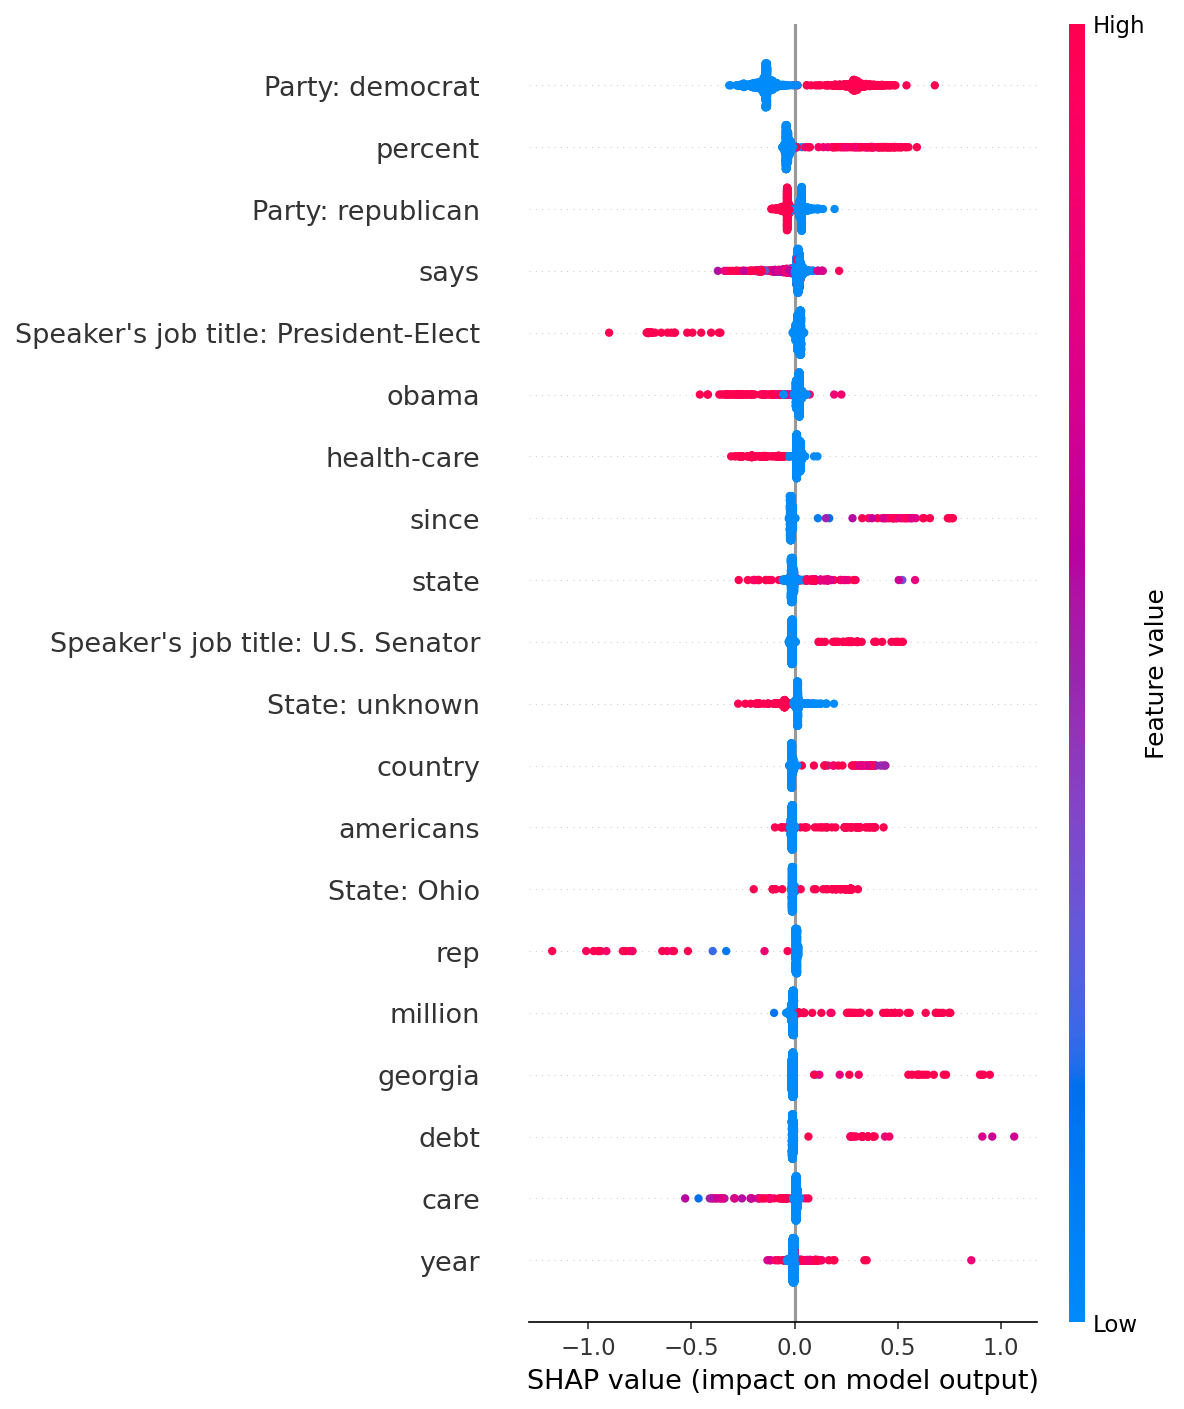
\includegraphics[width=\columnwidth]{figures/shap_beeswarm.png}
\caption{SHAP beeswarm plot showing the distribution and direction of each
feature's contribution across the test set.}
\label{fig:shap-beeswarm}
\end{figure}

\begin{figure}[!t]
\centering

\includegraphics[width=\columnwidth]{figures/shap_per_class.png}
\caption{Per-class SHAP breakdown: top features pushing toward \emph{fake} (red,
negative mean SHAP) vs.\ toward \emph{real} (blue, positive mean SHAP).}
\label{fig:shap-per-class}
\end{figure}

Figure~\ref{fig:shap-per-class} makes the bias concern concrete: \texttt{Party:
democrat} is among the strongest features pushing toward \emph{fake}, while
\texttt{Party: republican} pushes toward \emph{real}. Other top fake-pushing
features are largely entity/topic words (\emph{barack}, \emph{rep}, \emph{tom})
and a context value (\emph{a chain email}); top real-pushing features include
\emph{worth}, \emph{million}, \emph{wisconsin}, and \emph{Speaker's job title:
President-Elect}. None of these constitute a general-purpose deception signal --
they are properties of \emph{which speaker/topic} a statement concerns, which
reflects PolitiFact's fact-checking patterns over the dataset's collection period
at least as much as it reflects the truthfulness of the language itself.

\begin{figure}[!t]
\centering

\includegraphics[width=\columnwidth]{figures/shap_force_fake_example.png}
\caption{SHAP force plot, an example correctly classified as fake: ``Says John
McCain has done nothing to help the vets.''}
\label{fig:shap-force-fake}
\end{figure}

\begin{figure}[!t]
\centering

\includegraphics[width=\columnwidth]{figures/shap_force_real_example.png}
\caption{SHAP force plot, an example correctly classified as real: ``Building a
wall on the U.S.-Mexico border will take literally years.''}
\label{fig:shap-force-real}
\end{figure}

For completeness, Figures~\ref{fig:chi2-features} and \ref{fig:mi-features}
reproduce the original draft's Chi2/MI feature-importance plots on the corrected
labels, again with un-stemmed labels for readability.

\begin{figure}[!t]
\centering
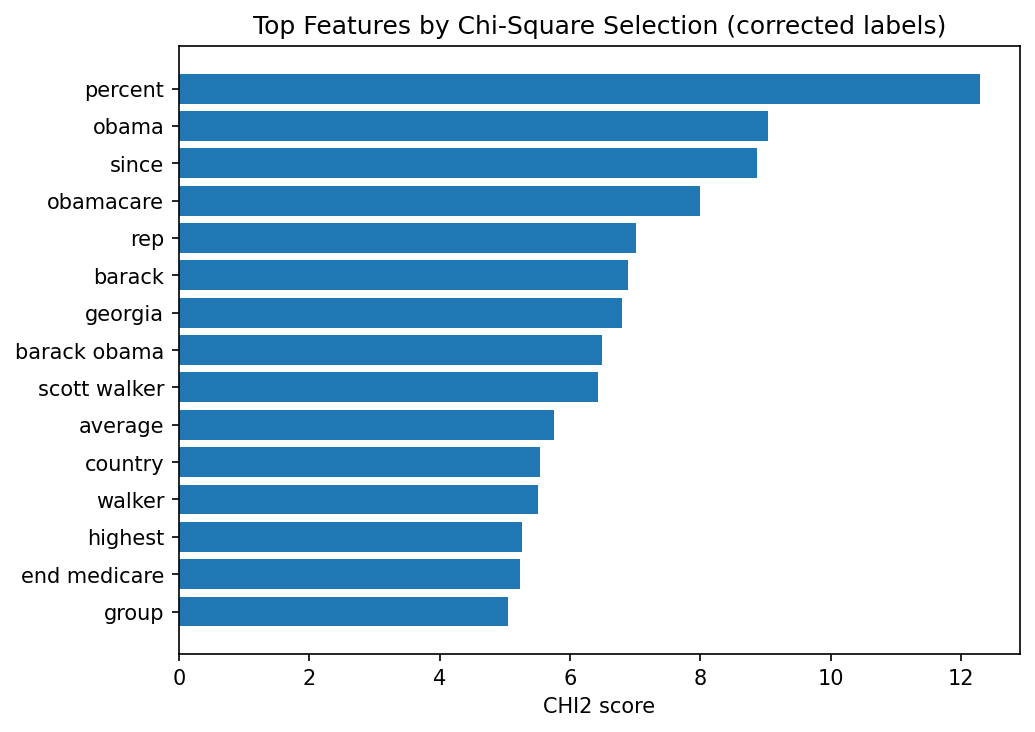
\includegraphics[width=\columnwidth]{figures/chi2_top_features.png}
\caption{Top 15 features by Chi-square score, corrected labels, un-stemmed
display labels.}
\label{fig:chi2-features}
\end{figure}

\begin{figure}[!t]
\centering
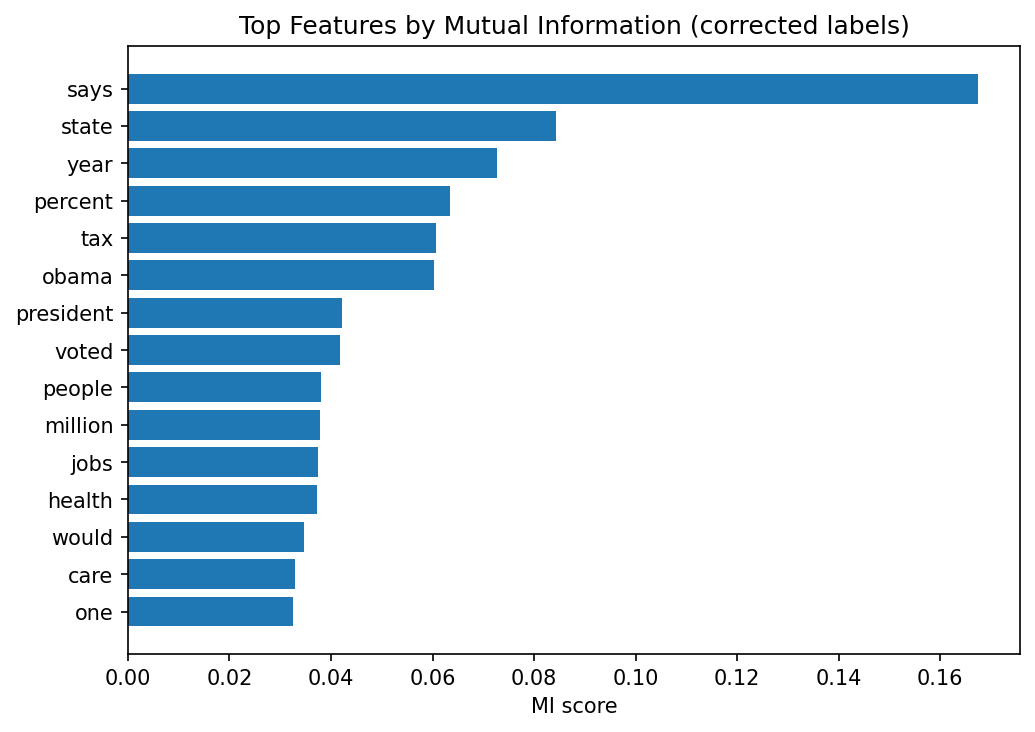
\includegraphics[width=\columnwidth]{figures/mi_top_features.png}
\caption{Top 15 features by Mutual Information score, corrected labels,
un-stemmed display labels.}
\label{fig:mi-features}
\end{figure}

\section{Limitations}
\textbf{Label integrity.} This paper's own history is itself a limitation worth
stating plainly: an initial implementation of this exact pipeline contained a
silent, case-sensitivity label-mapping defect that produced an invalid headline
result. The corrected pipeline adds a class-balance assertion specifically to
prevent silent recurrence, but this incident is a reminder that a plausible-looking
high score is not, by itself, evidence of correctness.

\textbf{Statistical power.} With $n=1{,}267$ test examples, several pipeline-stage
comparisons that look meaningful as point estimates (Section~VII-C) are not
statistically significant. Readers should treat any macro-F1 gap smaller than
roughly 0.03--0.04 between two configurations in this study as within noise unless
a significance test explicitly says otherwise.

\textbf{Topical/entity bias.} As shown in Section~VIII, the model's most
influential features are topical and entity-based (including party affiliation)
rather than general linguistic deception markers. This limits generalization to
new speakers, parties, or time periods outside the LIAR collection window, and
means the reported performance should not be read as evidence of a general fake
news detector.

\textbf{Domain and context.} As in the original draft, LIAR statements are short,
single-sentence, and restricted to U.S.\ political discourse; the models here do
not have access to broader document context or social/network signals that a
real-world deployment would likely require.

\textbf{Speaker exclusion.} Speaker identity is excluded from the recommended
pipeline based on both a theoretical leakage concern and an empirical null result
(Section~VII-B). This is a conservative choice that may discard some genuine
predictive signal along with the identity-memorization risk; it was not evaluated
against a fully anonymized alternative encoding.

\section{Conclusion}
This paper reproduced and corrected a label-mapping defect in an explainable fake
news detection pipeline built on the LIAR benchmark, and used the correction as an
opportunity to substantially strengthen the study's methodology: macro-F1 as the
primary metric, Dummy and class-weighted baselines, an actually-implemented
text+metadata feature space (rather than a claimed one), a leakage-safe
\texttt{scikit-learn} \texttt{Pipeline}, a controlled ablation with
cross-validated variance and McNemar significance testing, a bootstrap confidence
interval, a DistilBERT reference point, and a SHAP explainability analysis
reframed as a dataset-bias finding.

The honest result is that text+metadata with Chi-square feature selection
significantly improves over text-only Logistic Regression (macro-F1 0.628 vs.\
0.596, McNemar $p=0.034$), while further hyperparameter tuning, despite scoring
best under cross-validation, does not generalize and is statistically
indistinguishable from the text-only baseline on this test set. This is a more
modest claim than the original draft's F1 of 0.87, but it is the claim the
evidence actually supports, and macro-F1 in the 0.60--0.65 range is a normal,
publishable result for LIAR-binary classification with classical models.

Future work should pursue the metadata Option~A direction further (e.g.\
evaluating an anonymized or embedding-based speaker representation rather than
excluding speaker outright), extend the DistilBERT reference point to a full
fine-tuning sweep with its own significance testing against the classical
pipeline, and investigate whether the topical/entity bias identified in
Section~VIII can be mitigated with adversarial debiasing or explicit
speaker/party-invariant training objectives, rather than only reported as a
limitation.

\section*{Acknowledgment}
The author would like to express sincere gratitude to the Faculty of Engineering,
University of Moratuwa, for providing the opportunity and resources to conduct
this research. Special thanks are extended to the course instructors and academic
staff for their valuable guidance, support, and feedback throughout the study. The
author also acknowledges the creators of the LIAR dataset and the researchers
whose prior work contributed significantly to the development of this study.

\begin{thebibliography}{99}

\bibitem{conroy2015} N. Conroy, V. Rubin, and Y. Chen, ``Automatic deception detection: Methods for finding fake news,'' \emph{Proceedings of the Association for Information Science and Technology}, vol. 52, no. 1, pp. 1--4, 2015.

\bibitem{feng2012} S. Feng, R. Banerjee, and Y. Choi, ``Syntactic stylometry for deception detection,'' in \emph{Proc.\ 50th Annual Meeting of the Association for Computational Linguistics}, 2012, pp. 171--175.

\bibitem{shu2017} K. Shu, A. Sliva, S. Wang, J. Tang, and H. Liu, ``Fake News Detection on Social Media: A Data Mining Perspective,'' \emph{ACM SIGKDD Explorations Newsletter}, vol. 19, no. 1, pp. 22--36, 2017.

\bibitem{perezrosas2015} V. P\'erez-Rosas and R. Mihalcea, ``Experiments in open domain deception detection,'' in \emph{Proc.\ EMNLP}, 2015, pp. 1120--1125.

\bibitem{salton1988} G. Salton and C. Buckley, ``Term-weighting approaches in automatic text retrieval,'' \emph{Information Processing \& Management}, vol. 24, no. 5, pp. 513--523, 1988.

\bibitem{wang2017} W. Y. Wang, ``Liar, Liar Pants on Fire: A New Benchmark Dataset for Fake News Detection,'' in \emph{Proc.\ 55th Annual Meeting of the Association for Computational Linguistics (ACL)}, 2017, pp. 422--426.

\bibitem{ribeiro2016lime} M. T. Ribeiro, S. Singh, and C. Guestrin, ``Why Should I Trust You? Explaining the Predictions of Any Classifier,'' in \emph{Proc.\ 22nd ACM SIGKDD}, 2016, pp. 1135--1144.

\bibitem{lundberg2017shap} S. M. Lundberg and S.-I. Lee, ``A Unified Approach to Interpreting Model Predictions,'' in \emph{Advances in Neural Information Processing Systems (NeurIPS)}, 2017.

\bibitem{sharma2020} U. Sharma, S. Saran, and S. M. Patil, ``Fake News Detection Using Machine Learning Algorithms,'' \emph{International Journal of Creative Research Thoughts (IJCRT)}, vol. 8, no. 6, pp. 1394--1402, 2020.

\bibitem{mccallum1998nb} A. McCallum and K. Nigam, ``A comparison of event models for Naive Bayes text classification,'' in \emph{AAAI Workshop on Learning for Text Categorization}, 1998.

\bibitem{cortes1995svm} C. Cortes and V. Vapnik, ``Support-vector networks,'' \emph{Machine Learning}, vol. 20, no. 3, pp. 273--297, 1995.

\bibitem{bishop2006pattern} C. M. Bishop, \emph{Pattern Recognition and Machine Learning}. Springer, 2006.

\bibitem{breiman2001rf} L. Breiman, ``Random forests,'' \emph{Machine Learning}, vol. 45, no. 1, pp. 5--32, 2001.

\bibitem{chen2016xgboost} T. Chen and C. Guestrin, ``XGBoost: A scalable tree boosting system,'' in \emph{Proc.\ 22nd ACM SIGKDD}, 2016, pp. 785--794.

\bibitem{pedregosa2011sklearn} F. Pedregosa et al., ``Scikit-learn: Machine learning in Python,'' \emph{Journal of Machine Learning Research}, vol. 12, pp. 2825--2830, 2011.

\bibitem{quan_liar_kaggle} D. Quan, ``LIAR Dataset,'' Kaggle. [Online]. Available: https://www.kaggle.com/datasets/doanquanvietnamca/liar-dataset

\bibitem{yang1997featureselection} Y. Yang and J. O. Pedersen, ``A comparative study on feature selection in text categorization,'' in \emph{Proc.\ ICML}, 1997, pp. 412--420.

\bibitem{adadi2018peeking} A. Adadi and M. Berrada, ``Peeking inside the black-box: A survey on explainable artificial intelligence (XAI),'' \emph{IEEE Access}, vol. 6, pp. 52138--52160, 2018.

\bibitem{powers2011eval} D. Powers, ``Evaluation: From precision, recall and F-measure to ROC, informedness, markedness and correlation,'' \emph{Journal of Machine Learning Technologies}, vol. 2, no. 1, pp. 37--63, 2011.

\bibitem{devlin2019bert} J. Devlin, M.-W. Chang, K. Lee, and K. Toutanova, ``BERT: Pre-training of Deep Bidirectional Transformers for Language Understanding,'' in \emph{Proc.\ NAACL-HLT}, 2019, pp. 4171--4186.

\bibitem{sanh2019distilbert} V. Sanh, L. Debut, J. Chaumond, and T. Wolf, ``DistilBERT, a distilled version of BERT: smaller, faster, cheaper and lighter,'' \emph{arXiv preprint arXiv:1910.01108}, 2019.

\bibitem{kaliyar2021fakebert} R. K. Kaliyar, A. Goswami, and P. Narang, ``FakeBERT: Fake news detection in social media with a BERT-based deep learning approach,'' \emph{Multimedia Tools and Applications}, vol. 80, pp. 11765--11788, 2021.

\bibitem{mcnemar1947} Q. McNemar, ``Note on the sampling error of the difference between correlated proportions or percentages,'' \emph{Psychometrika}, vol. 12, no. 2, pp. 153--157, 1947.

\bibitem{efron1979bootstrap} B. Efron, ``Bootstrap methods: Another look at the jackknife,'' \emph{The Annals of Statistics}, vol. 7, no. 1, pp. 1--26, 1979.

\end{thebibliography}

\end{document}
